% Options for packages loaded elsewhere
\PassOptionsToPackage{unicode}{hyperref}
\PassOptionsToPackage{hyphens}{url}
%
\documentclass[
  11pt,
]{article}
\usepackage{amsmath,amssymb}
\usepackage{iftex}
\ifPDFTeX
  \usepackage[T1]{fontenc}
  \usepackage[utf8]{inputenc}
  \usepackage{textcomp} % provide euro and other symbols
\else % if luatex or xetex
  \usepackage{unicode-math} % this also loads fontspec
  \defaultfontfeatures{Scale=MatchLowercase}
  \defaultfontfeatures[\rmfamily]{Ligatures=TeX,Scale=1}
\fi
\usepackage{lmodern}
\ifPDFTeX\else
  % xetex/luatex font selection
  \setmainfont[]{DejaVu Serif}
\fi
% Use upquote if available, for straight quotes in verbatim environments
\IfFileExists{upquote.sty}{\usepackage{upquote}}{}
\IfFileExists{microtype.sty}{% use microtype if available
  \usepackage[]{microtype}
  \UseMicrotypeSet[protrusion]{basicmath} % disable protrusion for tt fonts
}{}
\makeatletter
\@ifundefined{KOMAClassName}{% if non-KOMA class
  \IfFileExists{parskip.sty}{%
    \usepackage{parskip}
  }{% else
    \setlength{\parindent}{0pt}
    \setlength{\parskip}{6pt plus 2pt minus 1pt}}
}{% if KOMA class
  \KOMAoptions{parskip=half}}
\makeatother
\usepackage{xcolor}
\usepackage[margin=1in]{geometry}
\usepackage{longtable,booktabs,array}
\usepackage{calc} % for calculating minipage widths
% Correct order of tables after \paragraph or \subparagraph
\usepackage{etoolbox}
\makeatletter
\patchcmd\longtable{\par}{\if@noskipsec\mbox{}\fi\par}{}{}
\makeatother
% Allow footnotes in longtable head/foot
\IfFileExists{footnotehyper.sty}{\usepackage{footnotehyper}}{\usepackage{footnote}}
\makesavenoteenv{longtable}
\usepackage{graphicx}
\makeatletter
\def\maxwidth{\ifdim\Gin@nat@width>\linewidth\linewidth\else\Gin@nat@width\fi}
\def\maxheight{\ifdim\Gin@nat@height>\textheight\textheight\else\Gin@nat@height\fi}
\makeatother
% Scale images if necessary, so that they will not overflow the page
% margins by default, and it is still possible to overwrite the defaults
% using explicit options in \includegraphics[width, height, ...]{}
\setkeys{Gin}{width=\maxwidth,height=\maxheight,keepaspectratio}
% Set default figure placement to htbp
\makeatletter
\def\fps@figure{htbp}
\makeatother
\setlength{\emergencystretch}{3em} % prevent overfull lines
\providecommand{\tightlist}{%
  \setlength{\itemsep}{0pt}\setlength{\parskip}{0pt}}
\setcounter{secnumdepth}{-\maxdimen} % remove section numbering
\ifLuaTeX
  \usepackage{selnolig}  % disable illegal ligatures
\fi
\IfFileExists{bookmark.sty}{\usepackage{bookmark}}{\usepackage{hyperref}}
\IfFileExists{xurl.sty}{\usepackage{xurl}}{} % add URL line breaks if available
\urlstyle{same}
\hypersetup{
  hidelinks,
  pdfcreator={LaTeX via pandoc}}

\author{}
\date{}

\begin{document}

\textbf{Drift-Sense: Machine-Learning Estimation of Short-Window IMU Position Drift}

Machine Learning course project report

\begin{longtable}[]{@{}
  >{\raggedright\arraybackslash}p{(\columnwidth - 2\tabcolsep) * \real{0.5769}}
  >{\raggedright\arraybackslash}p{(\columnwidth - 2\tabcolsep) * \real{0.4231}}@{}}
\toprule\noalign{}
\begin{minipage}[b]{\linewidth}\raggedright
\textbf{Team member}
\end{minipage} & \begin{minipage}[b]{\linewidth}\raggedright
\textbf{Enrollment ID}
\end{minipage} \\
\midrule\noalign{}
\endhead
\bottomrule\noalign{}
\endlastfoot
Guru Manohar Gupta & 2401010125 \\
Harsith Priyan & 2401010398 \\
Pranavi Mathur & 2401020046 \\
Yatin Singh & 2401010243 \\
Dadi Dinesh & 2401010136 \\
\end{longtable}

Project repository: https://github.com/Harsith-Panda/Drift-Sense {[}4{]}

Abstract

Drift-Sense studies whether motion statistics from an inertial measurement unit (IMU) can predict short-window position drift. The pipeline aligns two EuRoC Machine Hall flights with ground truth, builds two-second windows, constructs labels using strapdown integration and extracts 104 sensor features. A mean predictor, ordinary least squares (OLS), Ridge and Lasso are compared using leave-one-flight-out evaluation with blocked inner tuning. Committed results report a mean Lasso MAE of 0.0250 m (2.50 cm) and a mean fold R² of 0.756, compared with a baseline MAE of 0.0453 m. The 44.7\% reduction measures drift-prediction error; the system does not yet correct trajectories. Only two flights support these development results, so evaluation on unseen flights remains essential.

1. Problem Statement

A micro aerial vehicle (drone) can estimate its own motion by integrating the readings of its IMU. Angular rate from the gyroscope is integrated to track orientation, and specific force from the accelerometer is rotated into the world frame, corrected for gravity, and integrated twice to obtain velocity and position. Small sensor errors such as bias and noise are integrated as well, so the calculated position drifts away from the true position, and the drift grows quickly with time {[}5{]}, {[}6{]}.

A navigation system that relies on inertial dead-reckoning therefore benefits from knowing how much it can trust the inertial estimate at any moment. Estimating this typically requires ground truth or additional sensors such as cameras.

\textbf{Problem statement.} Given a short window (two seconds) of raw six-channel IMU data (gyroscope gx, gy, gz and accelerometer ax, ay, az) recorded on a micro aerial vehicle, predict the magnitude of the position drift that integrating that window would produce, using only features computed from the sensor readings themselves. This is a supervised regression task: the input consists of sensor-derived features and the target is a distance in meters. The model estimates the error of a particular short-window integration procedure.

\textbf{Objectives}

\begin{enumerate}
\def\labelenumi{\arabic{enumi}.}
\item
  Build a reproducible pipeline that turns EuRoC MAV flight recordings {[}1{]}, {[}2{]}, {[}3{]} into labeled two-second windows, where the label is the measured integration error against ground truth.
\item
  Summarize each window as a fixed set of statistical features (time-domain, frequency-domain and cross-axis).
\item
  Train and compare interpretable regression models (mean baseline, OLS, Ridge, Lasso) to predict the drift magnitude.
\item
  Evaluate honestly, using a split by flight rather than a random split of heavily overlapping windows, and report the limitations of the evidence.
\item
  Save a reusable scaler-plus-model pipeline.
\end{enumerate}

\textbf{An illustrative example.} Suppose the true endpoint is (5, 3, 2) m and IMU integration produces (6, 3, 2) m. The label is a drift magnitude of 1 m. If the ML model estimates 1.03 m, its absolute prediction error is 0.03 m. This example separates the physical drift being predicted from the regression error used to assess the model.

\textbf{Scope.} The work is offline and uses two EuRoC Machine Hall flights. The implementation reads recorded gyroscope and accelerometer data. The model estimates the size of the drift only: it does not correct the trajectory, does not use camera images (despite the visual-inertial context of the dataset), and has no live drone integration or live sensor ingestion. Although the Python package is named vio\_drift, the present experiment models IMU-only integration drift. The deep-learning and correction directories are placeholders.

2. Data and Preparation

2.1 Dataset

The experiment uses the EuRoC micro aerial vehicle (MAV) datasets {[}1{]}, {[}2{]}, distributed through the ETH Research Collection {[}3{]}. They were recorded on an Asctec Firefly hex-rotor carrying a visual-inertial sensor unit with a MEMS IMU (ADIS16448, angular rate and acceleration at 200 Hz) and stereo cameras (2 × 20 FPS). The Machine Hall recordings include millimeter-accurate position ground truth from a Leica MS50 laser tracker, and the dataset provides post-processed, spatio-temporally aligned ground truth {[}2{]}. This project uses only the IMU data and ground truth of the two ``easy'' Machine Hall flights, MH\_01\_easy and MH\_02\_easy; camera images are not used.

The dataset authors note that very dynamic motion can degrade laser-tracker accuracy (the effect at the start and end of each sequence is assumed negligible) and that synchronization between sensor data and ground truth is limited because they were recorded on different systems {[}2{]}. Because our labels are differences between integrated and ground-truth positions, ground-truth errors enter the labels and should be kept in mind when interpreting centimeter-level prediction errors.

Fig. 1 shows the ground-truth trajectories of the two flights used in this project.

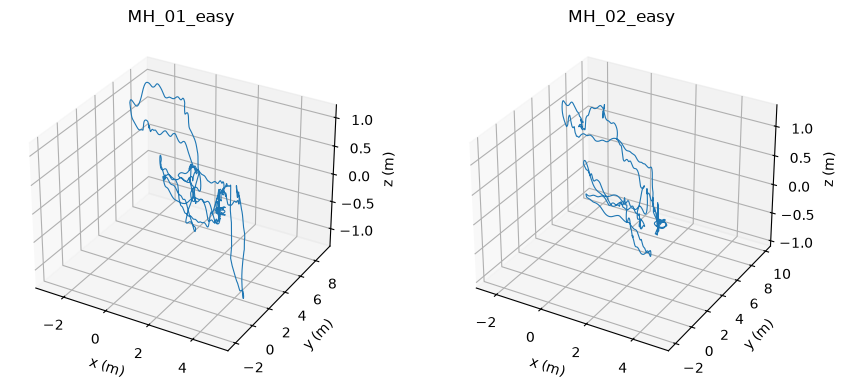
\includegraphics[width=5.39583in,height=2.48958in]{./media/66149f3a9585ec1b04c2e312f04e84cfdfce1942.png}

\emph{Fig. 1. Ground-truth 3-D trajectories of MH\_01\_easy (left) and MH\_02\_easy (right). Source: project repository {[}4{]}.}

2.2 Data quality

Each flight supplies IMU readings and ground-truth state estimates. The committed quality summary {[}4{]} records no missing values in the two raw streams and approximately 200 Hz sampling, consistent with the IMU rate stated in {[}2{]}.

\textbf{Table 1. Raw data, alignment and window counts}

\begin{longtable}[]{@{}
  >{\raggedright\arraybackslash}p{(\columnwidth - 4\tabcolsep) * \real{0.3846}}
  >{\raggedright\arraybackslash}p{(\columnwidth - 4\tabcolsep) * \real{0.3077}}
  >{\raggedright\arraybackslash}p{(\columnwidth - 4\tabcolsep) * \real{0.3077}}@{}}
\toprule\noalign{}
\begin{minipage}[b]{\linewidth}\raggedright
\textbf{Property}
\end{minipage} & \begin{minipage}[b]{\linewidth}\raggedright
\textbf{MH\_01\_easy}
\end{minipage} & \begin{minipage}[b]{\linewidth}\raggedright
\textbf{MH\_02\_easy}
\end{minipage} \\
\midrule\noalign{}
\endhead
\bottomrule\noalign{}
\endlastfoot
Raw IMU rows & 36,820 & 30,400 \\
Ground-truth rows & 36,382 & 29,993 \\
Recorded duration & 184.095 s & 151.995 s \\
Alignment rows dropped & 431 & 400 \\
Alignment drop rate & 1.17\% & 1.32\% \\
Two-second windows & 720 & 592 \\
\end{longtable}

2.3 Loading and timestamp alignment

loader.py expects seven IMU columns and seventeen ground-truth columns. It assigns project column names, converts timestamps to integers, sorts by timestamp and removes duplicates. Ground-truth quaternions are normalized. align.py uses a nearest-time merge and drops matches farther than 20 ms from an IMU timestamp. The signed matching gap remains available for inspection.

2.4 Window configuration

The current configuration uses a two-second duration and a 0.25-second stride. A window contains approximately 400 readings across six channels. Neighboring windows share 87.5 percent of their duration. Window creation uses timestamps rather than a fixed number of rows, while an expected-row check rejects windows with an excessive sample-count difference.

The raw-window array has shape (N, 400, 6), with channels ordered gx, gy, gz, ax, ay, az. Slight sample-count differences are padded with the final sample or truncated. The statistical feature code subsequently assumes a nominal 200 Hz rate for FFT and jerk calculations.

Fig. 2 shows an example of the raw gyroscope and accelerometer channels over the first ten seconds of MH\_01\_easy.

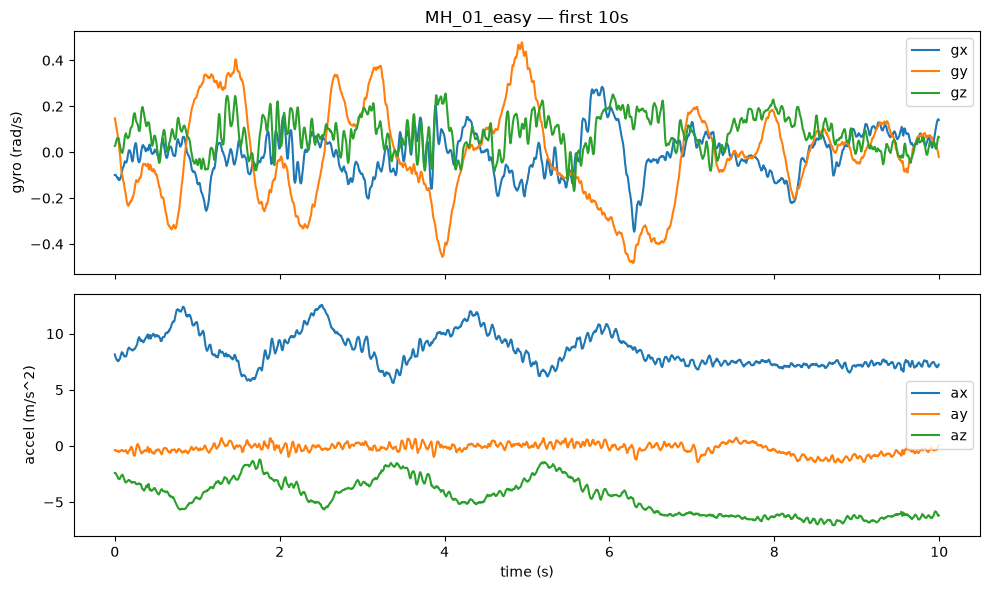
\includegraphics[width=4.60417in,height=2.73958in]{./media/b0c49fffc29928c9a05dddcc2a09896088b6d9df.png}

\emph{Fig. 2. Example raw IMU channels (gyroscope above, accelerometer below), first 10 s of MH\_01\_easy. Source: project repository {[}4{]}.}

3. System Architecture

Drift-Sense separates reusable functions in src/vio\_drift from command-line orchestration in scripts and explanatory experiments in notebooks. Files on disk form the interfaces between stages. The training path consumes statistical features and labels, while the physics-feature path supports separate diagnostics.

Fig. 3 summarizes the end-to-end pipeline, from raw EuRoC recordings to the saved final model.

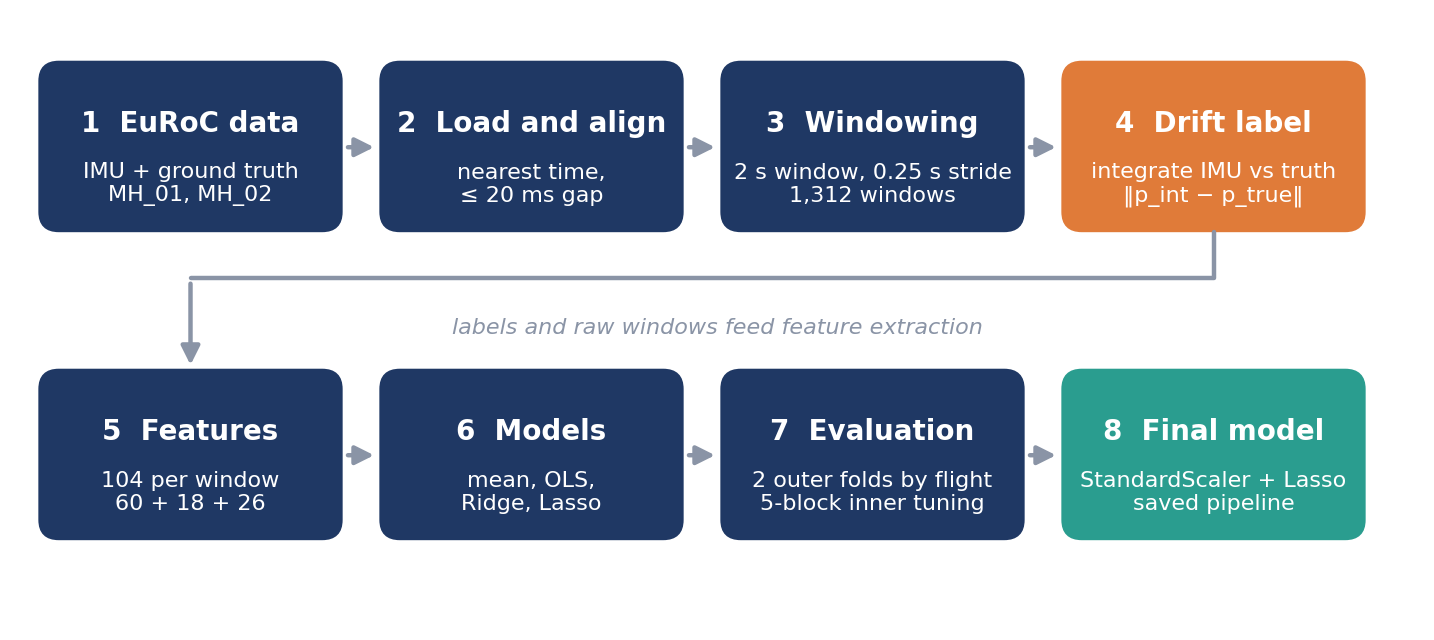
\includegraphics[width=6.39583in,height=2.85417in]{./media/9ff0932229f05eb945b7d27e7a7ef86c265e6e24.png}

\emph{Fig. 3. End-to-end Drift-Sense pipeline.}

\textbf{Table 2. Pipeline stages}

\begin{longtable}[]{@{}
  >{\raggedright\arraybackslash}p{(\columnwidth - 4\tabcolsep) * \real{0.2137}}
  >{\raggedright\arraybackslash}p{(\columnwidth - 4\tabcolsep) * \real{0.4444}}
  >{\raggedright\arraybackslash}p{(\columnwidth - 4\tabcolsep) * \real{0.3419}}@{}}
\toprule\noalign{}
\begin{minipage}[b]{\linewidth}\raggedright
\textbf{Stage}
\end{minipage} & \begin{minipage}[b]{\linewidth}\raggedright
\textbf{Implementation}
\end{minipage} & \begin{minipage}[b]{\linewidth}\raggedright
\textbf{Output}
\end{minipage} \\
\midrule\noalign{}
\endhead
\bottomrule\noalign{}
\endlastfoot
Load and align & data/loader.py, align.py & Aligned IMU and ground truth \\
Window and label & data/windowing.py, labels/ & Window labels and raw arrays \\
Extract features & features/, make\_features.py & 104 features per window \\
Fit and evaluate & models/ml/, train\_eval.py & Fold metrics and CV tables \\
Fit final model & train\_final.py & Lasso pipeline and metadata \\
\end{longtable}

3.1 Training data contracts

windows\_\textless sequence\textgreater.csv contains sequence and window identifiers, start and end timestamps, raw error magnitude and axis components, plus bias-corrected diagnostic labels. windows\_raw\_\textless sequence\textgreater.npy stores the raw sensor windows. features\_\textless sequence\textgreater.csv stores identifiers, the 104 unscaled features and the primary target. splits.json records the outer flight assignments.

3.2 Training and inference

During training, ground truth creates the target labels. The deployed statistical model accepts the 104 sensor features without ground-truth columns. Its saved StandardScaler applies the same preprocessing used during fitting. Inference must preserve feature names, order, units, sampling assumptions and window duration.

The final artifact is models/ml/lasso\_err\_mag\_m.pkl with a JSON metadata companion. The code provides a load-and-predict example, but a complete streaming inference service and input-quality checks are not yet implemented. The physics diagnostic has different assumptions because it uses ground-truth starting states and training-flight calibration biases.

4. Drift Label Construction

4.1 Starting state and orientation

For each window, drift\_label.py reads the first aligned ground-truth position p0, velocity v0 and quaternion q0. A quaternion represents three-dimensional orientation. The integrator starts from this reference state and then advances using the window's raw IMU measurements. Resetting every window isolates local integration error from drift accumulated before the window.

4.2 Integration equations

With the configured body-to-world rotation R(q), the acceleration update is a\_world = R(q) f\_body + g\_world. The gravity vector is (0, 0, −9.81) m/s². For each timestamp interval Δt, position updates as p\_next = p + v Δt + 0.5 a\_world Δt², and velocity updates as v\_next = v + a\_world Δt. A rotation increment derived from angular rate advances the quaternion, which is normalized after multiplication.

The implementation compares the predicted endpoint with ground truth at the final retained row. The configured interval is half-open, so a regular 400-sample window at 200 Hz spans approximately 1.995 seconds between its first and last samples. The nominal two-second duration describes window selection.

4.3 Raw error and diagnostic error

The signed vector error is e = p\_integrated − p\_true. Its components become err\_dx, err\_dy and err\_dz. The main regression label is err\_mag\_m = ‖e‖₂. It is nonnegative and measured in meters.

A second integration subtracts the dataset's per-row gyroscope and accelerometer bias estimates. The resulting err\_*\_bc fields form an oracle diagnostic. The saved mean residual magnitude is 0.0631 m for MH\_01\_easy and 0.0540 m for MH\_02\_easy, substantially below the raw means near 1.21 m {[}4{]}. This supports a strong bias contribution, consistent with the known sensitivity of inertial integration to sensor bias {[}5{]}, {[}6{]}, but does not establish a precise additive percentage decomposition of vector-error magnitude.

Fig. 4 compares raw and bias-corrected (oracle) drift for the two flights.

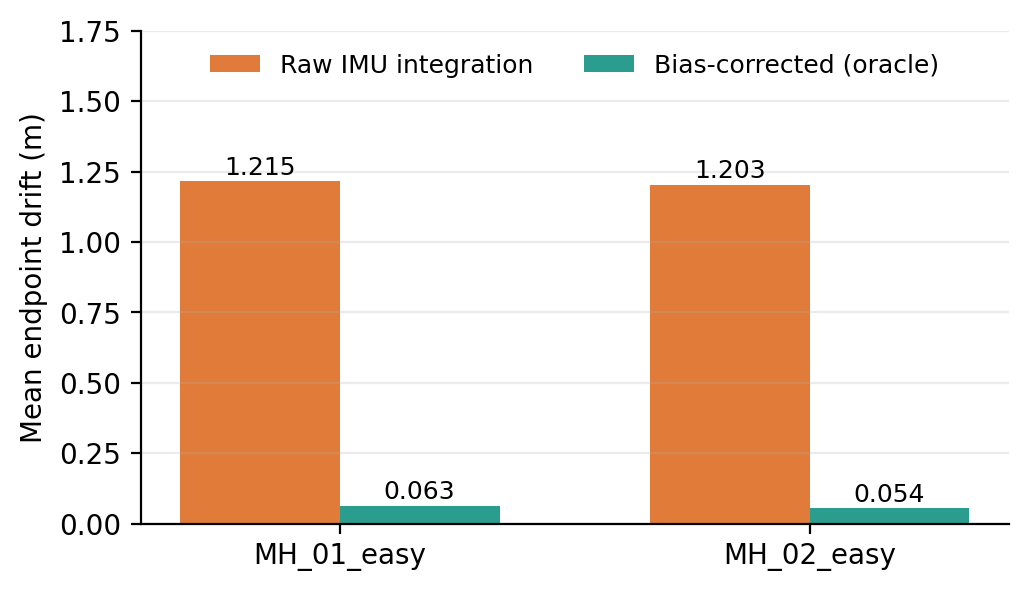
\includegraphics[width=4.60417in,height=2.64583in]{./media/4d412c537b400b466a116ed7b4003a8758b26e2f.png}

\emph{Fig. 4. Mean endpoint drift per two-second window: raw IMU integration versus the bias-corrected oracle diagnostic (values from the committed label summary).}

5. Feature Engineering

Each window becomes a vector of 104 numerical summaries. The feature families describe signal level, variation, frequency content and relationships between channels. Features use raw sensor readings, while ground-truth quantities remain outside the main statistical feature vector {[}4{]}.

\textbf{Table 3. Feature families}

\begin{longtable}[]{@{}
  >{\raggedright\arraybackslash}p{(\columnwidth - 4\tabcolsep) * \real{0.2564}}
  >{\raggedright\arraybackslash}p{(\columnwidth - 4\tabcolsep) * \real{0.1068}}
  >{\raggedright\arraybackslash}p{(\columnwidth - 4\tabcolsep) * \real{0.6368}}@{}}
\toprule\noalign{}
\begin{minipage}[b]{\linewidth}\raggedright
\textbf{Family}
\end{minipage} & \begin{minipage}[b]{\linewidth}\raggedright
\textbf{Count}
\end{minipage} & \begin{minipage}[b]{\linewidth}\raggedright
\textbf{Examples and meaning}
\end{minipage} \\
\midrule\noalign{}
\endhead
\bottomrule\noalign{}
\endlastfoot
Time domain & 60 & Ten statistics on each of six channels \\
Frequency domain & 18 & Dominant frequency, energy and entropy per channel \\
Cross axis and magnitude & 26 & Vector magnitudes, jerk and fifteen correlations \\
Total & 104 & \\
\end{longtable}

5.1 Time-domain statistics

For each channel, time\_domain.py calculates mean, standard deviation, variance, RMS, minimum, maximum, peak-to-peak range, skewness, excess kurtosis and mean-centered zero-crossing rate. Centering zero crossings avoids letting a gravity offset dominate that feature. Constant channels receive zero skewness and kurtosis.

5.2 Frequency and cross-axis statistics

frequency\_domain.py removes the channel mean, computes a real FFT and summarizes dominant frequency, summed spectral energy and normalized spectral entropy. cross\_axis.py computes acceleration and gyroscope magnitudes, finite-difference jerk at 200 Hz, and Pearson correlations for every channel pair. Undefined correlations for constant channels become zero.

5.3 Scaling and redundancy

Features have different units and scales. StandardScaler fits only on training rows inside each model pipeline, including inside cross-validation. Related features can be highly correlated, such as standard deviation and variance. Regularization reduces the instability that can arise when a linear model fits many correlated predictors to a small number of independent flights {[}9{]}.

6. Models and Evaluation

\textbf{Table 4. Models compared}

\begin{longtable}[]{@{}
  >{\raggedright\arraybackslash}p{(\columnwidth - 2\tabcolsep) * \real{0.2991}}
  >{\raggedright\arraybackslash}p{(\columnwidth - 2\tabcolsep) * \real{0.7009}}@{}}
\toprule\noalign{}
\begin{minipage}[b]{\linewidth}\raggedright
\textbf{Model}
\end{minipage} & \begin{minipage}[b]{\linewidth}\raggedright
\textbf{Training behavior}
\end{minipage} \\
\midrule\noalign{}
\endhead
\bottomrule\noalign{}
\endlastfoot
Mean baseline & Predicts the training label mean for every window \\
Ordinary least squares & Fits a linear combination of standardized features \\
Ridge regression & Adds an L2 penalty to shrink coefficient magnitudes {[}8{]} \\
Lasso regression & Adds an L1 penalty and can set coefficients to zero {[}7{]} \\
\end{longtable}

For a feature vector x, the linear prediction is ŷ = wᵀx + b. OLS minimizes squared error. Ridge adds α‖w‖₂² to the summed squared loss. scikit-learn's Lasso {[}10{]} uses (1/2n) times the summed squared loss plus α‖w‖₁. The alpha grids contain 17 Ridge values from 10⁻³ to 10⁵ and 16 Lasso values from 10⁻⁶ to 10⁻¹. All models are implemented with scikit-learn {[}10{]}.

6.1 Outer flight split

The first fold trains on MH\_02\_easy and tests on MH\_01\_easy. The second reverses those roles. This prevents the heavily overlapping windows of one recording from appearing on both sides of the outer split. The number of independent flights remains two, even though the dataset contains 1,312 overlapping examples.

6.2 Inner tuning

Within each outer fold, the training flight is divided into five contiguous blocks. Each block serves as validation once, with the other blocks used for fitting. Sixteen nearby windows on either side are purged from training. At the current stride this is a four-second exclusion, exceeding the two-second window duration.

The implemented selection rule chooses the alpha with the lowest median block MAE. It reduces the influence of the unusually difficult early-flight block. The code also reports mean-error and one-standard-error selections. The median rule changes which operating segments influence tuning and therefore needs evaluation on independent flights.

6.3 Metrics and interpretation

MAE is the average absolute difference between predicted and true drift magnitude. RMSE gives larger residuals more weight. R² measures squared-error improvement relative to predicting the test set's own mean. Prediction bias is the mean of prediction minus target. Results average metrics equally across the two folds rather than pooling all windows.

6.4 Evaluation qualification

Diagnostic scripts compared window lengths and tuning rules using these same flights {[}4{]}. Their use in design selection means the reported scores are development results rather than a final untouched benchmark. A new flight-level test set is needed after freezing preprocessing, model selection and tuning rules.

7. Results and Error Analysis

The committed results {[}4{]} identify Lasso as the best of the four main models by mean held-out MAE. Table 5 reports equal-weight averages over the two outer folds. The values describe prediction of local raw-IMU drift magnitude.

\textbf{Table 5. Held-out results (mean of two outer folds)}

\begin{longtable}[]{@{}
  >{\raggedright\arraybackslash}p{(\columnwidth - 6\tabcolsep) * \real{0.3590}}
  >{\raggedright\arraybackslash}p{(\columnwidth - 6\tabcolsep) * \real{0.2137}}
  >{\raggedright\arraybackslash}p{(\columnwidth - 6\tabcolsep) * \real{0.2137}}
  >{\raggedright\arraybackslash}p{(\columnwidth - 6\tabcolsep) * \real{0.2137}}@{}}
\toprule\noalign{}
\begin{minipage}[b]{\linewidth}\raggedright
\textbf{Model}
\end{minipage} & \begin{minipage}[b]{\linewidth}\raggedright
\textbf{MAE (cm)}
\end{minipage} & \begin{minipage}[b]{\linewidth}\raggedright
\textbf{RMSE (cm)}
\end{minipage} & \begin{minipage}[b]{\linewidth}\raggedright
\textbf{Mean R²}
\end{minipage} \\
\midrule\noalign{}
\endhead
\bottomrule\noalign{}
\endlastfoot
Mean baseline & 4.53 & 6.91 & −0.032 \\
OLS & 2.99 & 4.15 & 0.580 \\
Ridge & 2.70 & 3.49 & 0.717 \\
\textbf{Lasso} & \textbf{2.50} & \textbf{3.23} & \textbf{0.756} \\
\end{longtable}

The relative MAE reduction is (0.0452505 − 0.0250447) / 0.0452505 ≈ 44.7 percent. Lasso's fold MAEs are approximately 2.59 cm on MH\_01\_easy and 2.42 cm on MH\_02\_easy. Its mean prediction bias is approximately −0.12 cm.

Fig. 5 plots the same held-out metrics as Table 5.

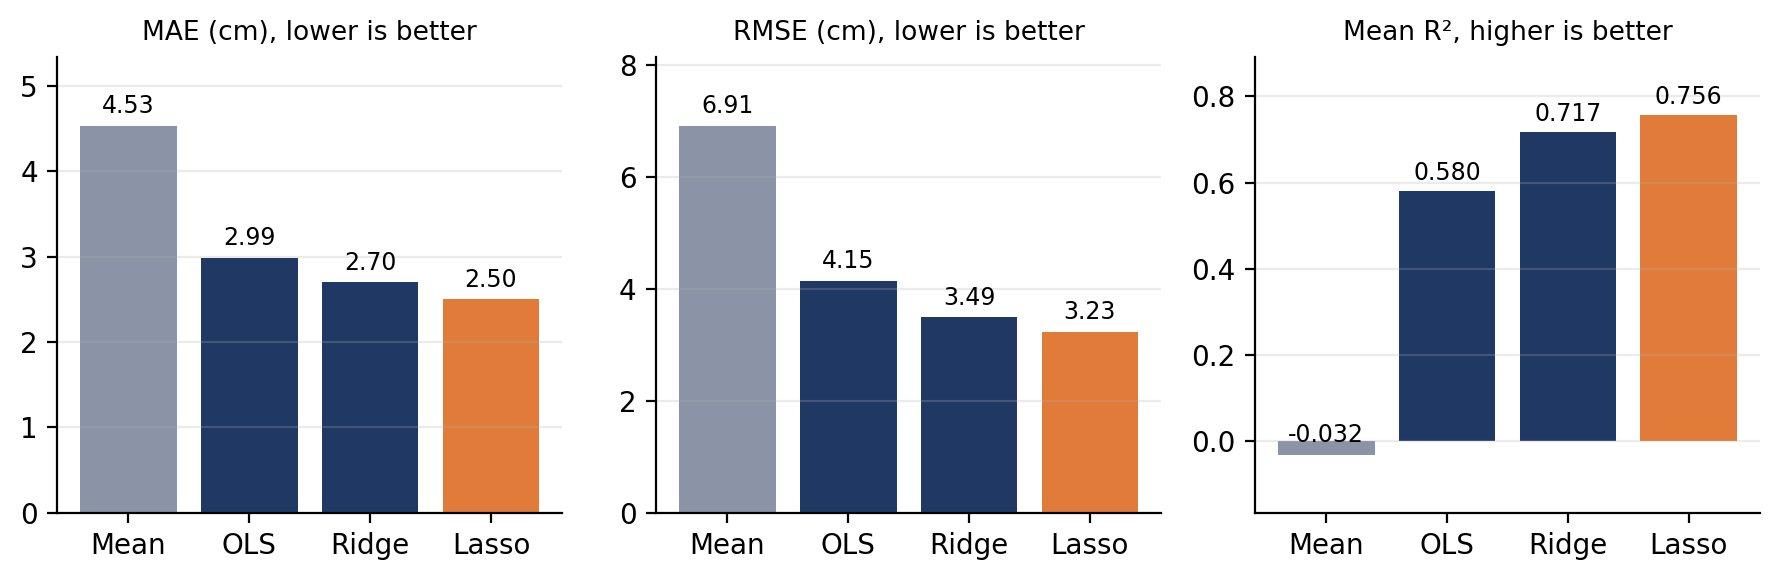
\includegraphics[width=6.39583in,height=2.08333in]{./media/ce1eec47c1afa705642fb9141d29c7d861d5fa29.png}

\emph{Fig. 5. Held-out MAE, RMSE and mean R² for the four models (values from Table 5).}

\emph{{[}Insert Fig. 6 here: notebook output for MH\_02\_easy showing true and predicted drift over time{]}}

\emph{Fig. 6. Committed notebook output for MH\_02\_easy showing true and predicted drift over time. Source: project repository {[}4{]}.}

7.1 Generalization and flight segments

OLS has the largest gap between training and held-out MAE. Its held-out to training ratio is approximately 1.81, compared with 1.38 for Ridge and 1.24 for Lasso. These results support regularization within this limited experiment.

The report's segment analysis shows Lasso R² of 0.86 and 0.84 in the first fifth of the two flights, but only 0.10 and 0.17 in the remaining portions. The model follows the large early-flight drift change more successfully than rapid fluctuations during normal flight. A whole-flight R² of 0.756 should therefore be interpreted alongside segment-level performance.

Fig. 7 shows this segment-level difference.

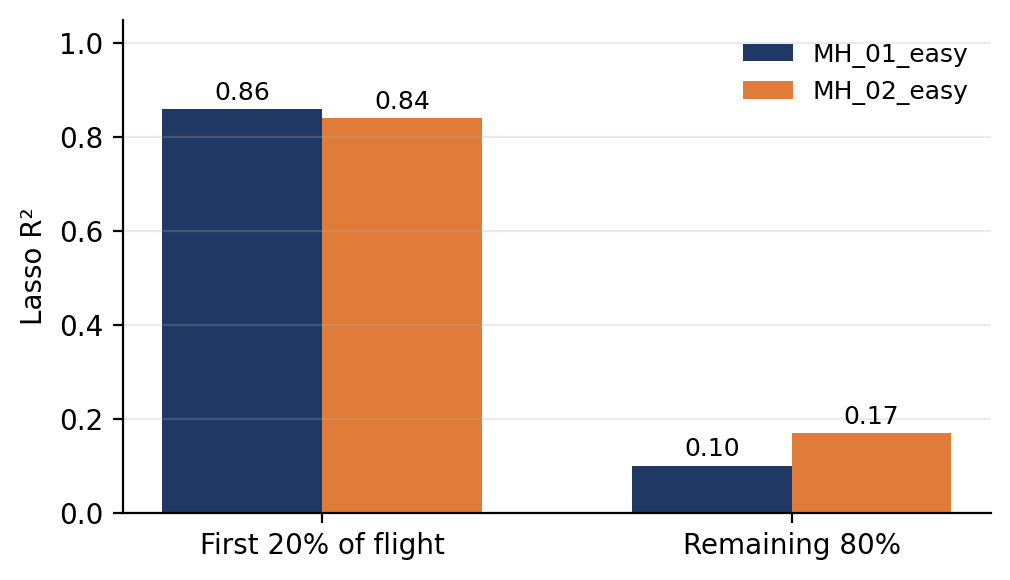
\includegraphics[width=4.60417in,height=2.64583in]{./media/5720d69a03f8af42c0474db666b60159b0379d05.png}

\emph{Fig. 7. Lasso R² in the first 20\% and the remaining 80\% of each held-out flight.}

8. Final Model

train\_final.py chooses alpha using leave-one-flight-out validation over both available flights, then refits Lasso on every window. The saved JSON records alpha = 0.0046415888, 1,312 windows, 104 input features and seven nonzero coefficients {[}4{]}. Because the final model uses both flights for fitting, its training score is not an independent generalization measurement.

\textbf{Table 6. Features retained by the final Lasso}

\begin{longtable}[]{@{}
  >{\raggedright\arraybackslash}p{(\columnwidth - 2\tabcolsep) * \real{0.2991}}
  >{\raggedright\arraybackslash}p{(\columnwidth - 2\tabcolsep) * \real{0.7009}}@{}}
\toprule\noalign{}
\begin{minipage}[b]{\linewidth}\raggedright
\textbf{Retained feature}
\end{minipage} & \begin{minipage}[b]{\linewidth}\raggedright
\textbf{Interpretation}
\end{minipage} \\
\midrule\noalign{}
\endhead
\bottomrule\noalign{}
\endlastfoot
gx\_max & Largest x-axis angular-rate reading \\
gy\_mean & Mean y-axis angular rate \\
ax\_rms & RMS of x-axis specific force \\
az\_mean & Mean z-axis specific force \\
gz\_dom\_freq & Dominant frequency of z-axis angular rate \\
az\_spec\_entropy & Frequency spread of z-axis specific force \\
corr\_ax\_az & Correlation of x and z accelerometer channels \\
\end{longtable}

The saved pipeline retains the 104-feature input schema. Applications must supply the complete expected feature list in order, even though most Lasso coefficients are zero.

9. Limitations and Conclusion

9.1 Scientific limitations

Only two easy flights from a shared sensor setting support the current results. Overlapping windows are correlated, so the row count overstates the amount of independent evidence. The label measures a locally reset integrator and uses ground-truth initialization. Broader claims about continuous navigation, aggressive motion or a different IMU require separate experiments.

The model outputs a scalar magnitude, which alone cannot specify the direction of a position correction. A correction system would need signed error components or another directional estimate and must demonstrate improved trajectories over time. No such corrected-trajectory result is currently implemented.

9.2 Engineering improvements

First, preserve window IDs consistently after label filtering and correct quaternion propagation in the alternate rotation branch. Second, update the remaining one-second documentation to the active two-second configuration. Third, strengthen semantic input validation and stop suppressing all training warnings. The hard-coded cross-validation gap should derive from window and stride settings when those become configurable.

\textbf{Table 7. Next work}

\begin{longtable}[]{@{}
  >{\raggedright\arraybackslash}p{(\columnwidth - 4\tabcolsep) * \real{0.0748}}
  >{\raggedright\arraybackslash}p{(\columnwidth - 4\tabcolsep) * \real{0.4487}}
  >{\raggedright\arraybackslash}p{(\columnwidth - 4\tabcolsep) * \real{0.4765}}@{}}
\toprule\noalign{}
\begin{minipage}[b]{\linewidth}\raggedright
\textbf{No.}
\end{minipage} & \begin{minipage}[b]{\linewidth}\raggedright
\textbf{Next work}
\end{minipage} & \begin{minipage}[b]{\linewidth}\raggedright
\textbf{Evidence required}
\end{minipage} \\
\midrule\noalign{}
\endhead
\bottomrule\noalign{}
\endlastfoot
1 & Freeze pipeline and test new flights & MAE and R² per unseen flight and segment \\
2 & Compare physics and nonlinear models & Same data splits and input assumptions \\
3 & Model signed axis errors & Direction accuracy and residual analysis \\
4 & Evaluate trajectory correction & Reduced continuous trajectory error \\
5 & Explore temporal deep learning & Independent gains over simpler baselines \\
\end{longtable}

9.3 Conclusion

Drift-Sense implements an interpretable supervised pipeline for predicting short-window IMU integration error. The saved experiments show that Lasso improves on a mean baseline and unregularized regression on the two available flights. The project's strongest demonstrated outcome is a reproducible feature and regression workflow, accompanied by useful diagnostics. Further validation should focus on untouched flights, realistic initialization and consistent evaluation before extending to live drift monitoring or correction.

References

{[}1{]} M. Burri, J. Nikolic, P. Gohl, T. Schneider, J. Rehder, S. Omari, M. W. Achtelik, and R. Siegwart, ``The EuRoC micro aerial vehicle datasets,'' The International Journal of Robotics Research, vol. 35, no. 10, pp. 1157--1163, 2016, doi: 10.1177/0278364915620033.

{[}2{]} ETH Zurich Autonomous Systems Lab, ``The EuRoC MAV Dataset,'' 2016. https://projects.asl.ethz.ch/datasets/euroc-mav/ (accessed Oct. 27, 2026). Dataset DOI: 10.3929/ethz-b-000690084.

{[}3{]} ETH Zurich, ``EuRoC MAV Dataset,'' ETH Research Collection (research data). https://www.research-collection.ethz.ch/entities/researchdata/bcaf173e-5dac-484b-bc37-faf97a594f1f (accessed Oct. 27, 2026).

{[}4{]} G. M. Gupta, H. Priyan, P. Mathur, Y. Singh, and D. Dinesh, ``Drift-Sense,'' GitHub repository (source code, committed results, notebooks and saved model metadata). https://github.com/Harsith-Panda/Drift-Sense (accessed Oct. 27, 2026).

{[}5{]} O. J. Woodman, ``An introduction to inertial navigation,'' University of Cambridge Computer Laboratory, Tech. Rep. UCAM-CL-TR-696, 2007.

{[}6{]} D. H. Titterton and J. L. Weston, Strapdown Inertial Navigation Technology, 2nd ed. Institution of Electrical Engineers, 2004.

{[}7{]} R. Tibshirani, ``Regression shrinkage and selection via the lasso,'' Journal of the Royal Statistical Society: Series B, vol. 58, no. 1, pp. 267--288, 1996.

{[}8{]} A. E. Hoerl and R. W. Kennard, ``Ridge regression: biased estimation for nonorthogonal problems,'' Technometrics, vol. 12, no. 1, pp. 55--67, 1970.

{[}9{]} T. Hastie, R. Tibshirani, and J. Friedman, The Elements of Statistical Learning, 2nd ed. Springer, 2009.

{[}10{]} F. Pedregosa et al., ``Scikit-learn: Machine learning in Python,'' Journal of Machine Learning Research, vol. 12, pp. 2825--2830, 2011.

\end{document}
